\section{Технологическая часть}

\subsection{Выбор языка программирования}
В качестве языка программирования был выбран С \cite{c}. Для сборки модуля использовалась утилита make.

Была выбрана среда разработки Visual Studio Code \cite{VStudio}, так как она бесплатная, кроссплатформенная,  а также позволяет использовать все возможности консоли, не переключаясь между окнами. \newline

\subsection{Структура загружаемого модуля}
Реализованный модуль включает в себя следующие функции:
\begin{itemize}
	\item \textbf{fw\_init()} -- функция инициализации модуля;
	
	\item \textbf{fw\_exit()}-- функция выгрузки модуля;
	
	\item \textbf{hide()} -- функция изменения видимости модуля (скрытие);
	
	\item \textbf{unhide()} -- функция изменения видимости модуля (обнаружение);
	
	\item \textbf{fw\_read(struct file *filp, char \_\_user *buff, size\_t count, loff\_t *f\_pos)} -- функция чтения, описываемая в структуре struct file\_operations;
	
	\item \textbf{fw\_write(struct file *filp, const char \_\_user *buff, size\_t count, loff\_t *f\_pos)} -- функция записи, описываемая в структуре struct file\_operations;
	
	\item \textbf{add\_rule(struct fw\_rule *rule)} -- добавление нового правила;
	
	\item \textbf{del\_rule(struct fw\_rule *rule)} -- удаление правила;
	
	\item \textbf{fw\_in\_filter(void *priv, struct sk\_buff *skb, const struct nf\_hook\_state *state)} -- <<обёртка>> функции фильтрации для входящих пакетов;
	
	\item \textbf{fw\_out\_filter(void *priv, struct sk\_buff *skb, const struct nf\_hook\_state *state)} -- <<обёртка>> функции фильтрации для исходящих пакетов;
	
	\item \textbf{filter(void *priv, struct sk\_buff *skb, const struct nf\_hook\_state *state,
	struct list\_head *list\_rule)} -- основная функция фильтрации пакетов;
	
	\item \textbf{str\_rule(struct fw\_rule *rule)} -- функция преобразования правила фильтрации в удобный для восприятия человеком вид;
	
	\item \textbf{str\_packet(uint32\_t src\_ip, uint16\_t src\_port,uint32\_t dest\_ip, uint16\_t \, dest\_port, char *protocol\_str)} -- функция преобразования информации о перехваченном пакете в удобный для восприятия человеком вид.
\end{itemize}
%
Были также определены структуры:
%
\begin{itemize}
	\item struct file\_operations;
	
	\item struct miscdevice;
	
	\item struct nf\_hook\_ops. \newline
\end{itemize}

\subsection{Структура проекта}
Проект состоит из нескольких частей (Рисунок \ref{fig30:image}).
\begin{figure}[h!]
	\begin{center}
		{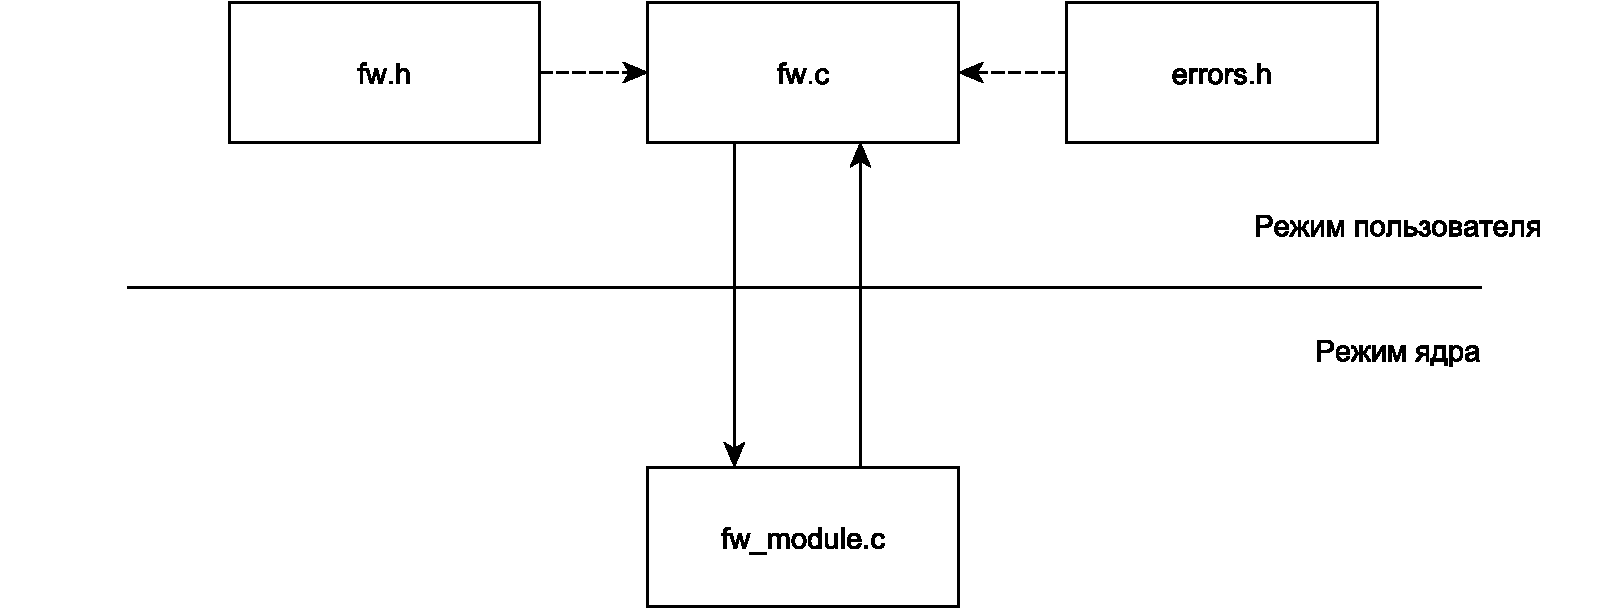
\includegraphics[scale = 0.63]{img/struct.pdf}}
		\caption{Структура ПО}
		\label{fig30:image}
	\end{center}
\end{figure}

В Приложении А представлены листинги каждой из частей проекта. \newline

\subsection{Сборка и запуск модуля}
Сборка модуля осуществляется командой make. На Листинге \ref{lst:make} приведено содержимое Makefile.

\begin{lstlisting}[caption = {Makefile}, label=lst:make]
obj-m += fw_module.o

all: fw.o fw_module.o

fw.o: fw.c fw.h
	gcc -o fw.o fw.c	

fw_module.o: fw_module.c
	make -C /lib/modules/$(shell uname -r)/build M=$(PWD) modules

clean:
	rm -rf fw *.o
	make -C /lib/modules/$(shell uname -r)/build M=$(PWD) clean
\end{lstlisting}

Для того, чтобы загрузить модуль, нужно воспользоваться командой \textbf{sudo insmod fw\_module.ko}, для того, чтобы выгрузить -- \textbf{sudo rmmod fw\_module}. \newline

\subsection{Алгоритм фильтрации пакетов}
На Листинге \ref{lst:filter} приведена реализация основного алгоритма фильтрации пакетов, описанного в параграфе \ref{sec:filter}. 
\begin{lstlisting}[caption = {Реализация алгоритма фильтрации пакетов}, label=lst:filter]
static unsigned int filter(void *priv, struct sk_buff *skb, const struct nf_hook_state *state, struct list_head *list_rule)
{
	struct iphdr *iph;
	struct tcphdr *tcph;
	struct udphdr *udph;
	
	unsigned char protocol;
	char *protocol_str;
	uint32_t src_ip, dest_ip;
	uint16_t src_port = NOT_STATED, dest_port = NOT_STATED;
	
	struct list_head *lst;
	struct rule_item *node;
	struct fw_rule *rule;
	
	if (!skb || list_rule->next == list_rule)
		return NF_ACCEPT;
	
	iph = (struct iphdr *)skb_network_header(skb);
	if (iph == NULL)
		return NF_ACCEPT;
	
	protocol = iph->protocol;
	src_ip = iph->saddr;
	dest_ip = iph->daddr;
	
	if (protocol == IPPROTO_UDP)
	{
		udph = (struct udphdr *)(skb_transport_header(skb));
		src_port = udph->source;
		dest_port = udph->dest;
		protocol_str = "UDP";
	}
	else if (protocol == IPPROTO_TCP)
	{
		tcph = (struct tcphdr *)(skb_transport_header(skb));
		src_port = tcph->source;
		dest_port = tcph->dest;
		protocol_str = "TCP";
	}
	else
		protocol_str = "-";
	
	lst = list_rule;
	list_for_each_entry(node, lst, list)
	{       
		rule = &node->rule; 
		
		if (rule->protocol != NOT_STATED && rule->protocol != iph->protocol)
			continue;
		if (rule->src_ip != NOT_STATED && !SAME_ADDR(rule->src_ip, src_ip))
			continue;	
		if (rule->dest_ip != NOT_STATED && !SAME_ADDR(rule->dest_ip, dest_ip))
			continue;
		if (rule->src_port != NOT_STATED && rule->src_port != src_port)
			continue;
		if (rule->dest_port != NOT_STATED && rule->dest_port != dest_port)
			continue;
		
		printk(KERN_INFO ">>> FIREWALL: packet was dropped. Details: %s", str_packet(src_ip, src_port, dest_ip, dest_port, protocol_str));
		
		return NF_DROP;
	}
	
	return NF_ACCEPT;
}

static unsigned int fw_in_filter(void *priv, struct sk_buff *skb, const struct nf_hook_state *state)
{
	return filter(priv, skb, state, &in_list);
}

static unsigned int fw_out_filter(void *priv, struct sk_buff *skb, const struct nf_hook_state *state)
{
	return filter(priv, skb, state, &out_list);
}
\end{lstlisting}

\subsection{Выводы}
Был выбран язык программирования и среда разработки, описана общая структура модуля и программного обеспечения, а также приведёна реализация основного алгоритма.